
%----------------------------------------------------------------------------
\chapter{Fejlesztést segítő eszközök}
%----------------------------------------------------------------------------
%----------------------------------------------------------------------------
\section{Continuous Integration}
%----------------------------------------------------------------------------
A fejlesztés során 

\begin{figure}[!ht]
  \centering
  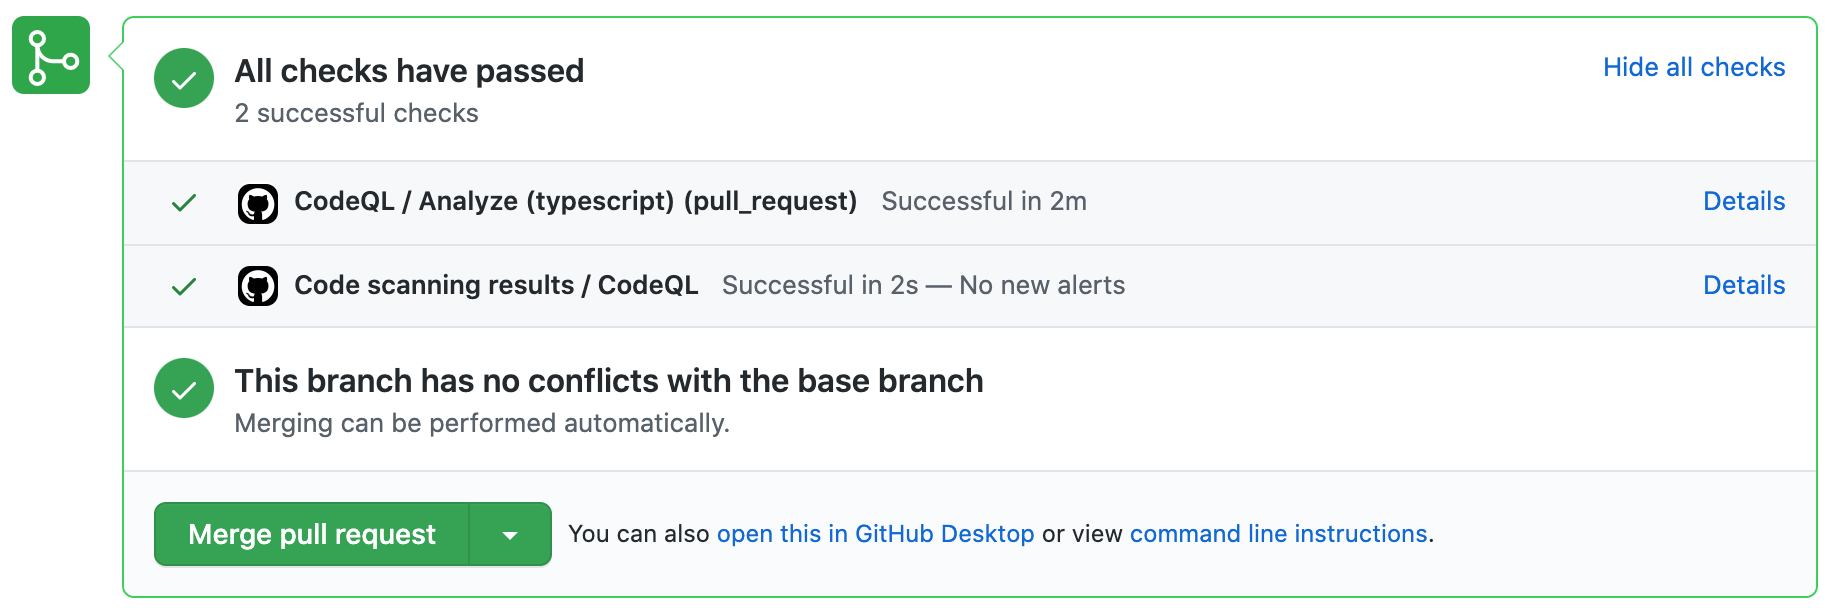
\includegraphics[width=150mm, keepaspectratio]{figures/ci.png}
  \caption{GitHub Action működés közben}
  \label{fig:GitHubAction}
\end{figure}

%----------------------------------------------------------------------------
\subsection{Linter}
%----------------------------------------------------------------------------

%----------------------------------------------------------------------------
\subsection{Statikus kódellenörzés}
%----------------------------------------------------------------------------

%----------------------------------------------------------------------------
\section{Continuous Deployment}
%----------------------------------------------------------------------------

%----------------------------------------------------------------------------
\subsection{Heroku}
%----------------------------------------------------------------------------

%----------------------------------------------------------------------------
\subsection{Vercel}
%----------------------------------------------------------------------------
